% TREE SPACE
\begin{frame}[plain]
\frametitle{Tree space as a hilly landscape}

\small{The space of all possible trees can be visualized as a hilly landscape. Nearby points in this landscape represent similar trees, and the height of the landscape is the probability of the tree at that point.}

\begin{columns}

\column{0.55\textwidth}

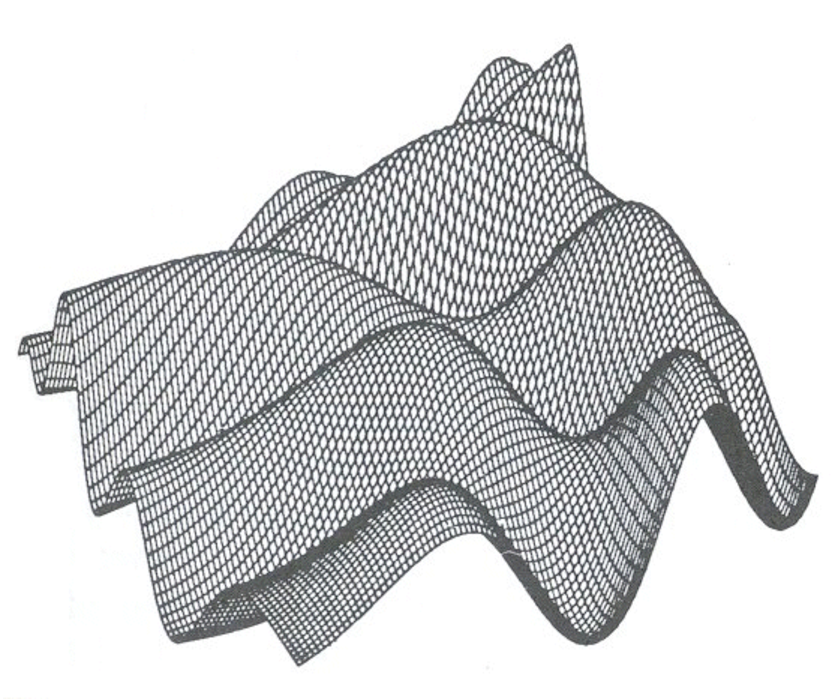
\includegraphics[width=\textwidth]{../images/hillyLandscape1}

\column{0.45\textwidth}

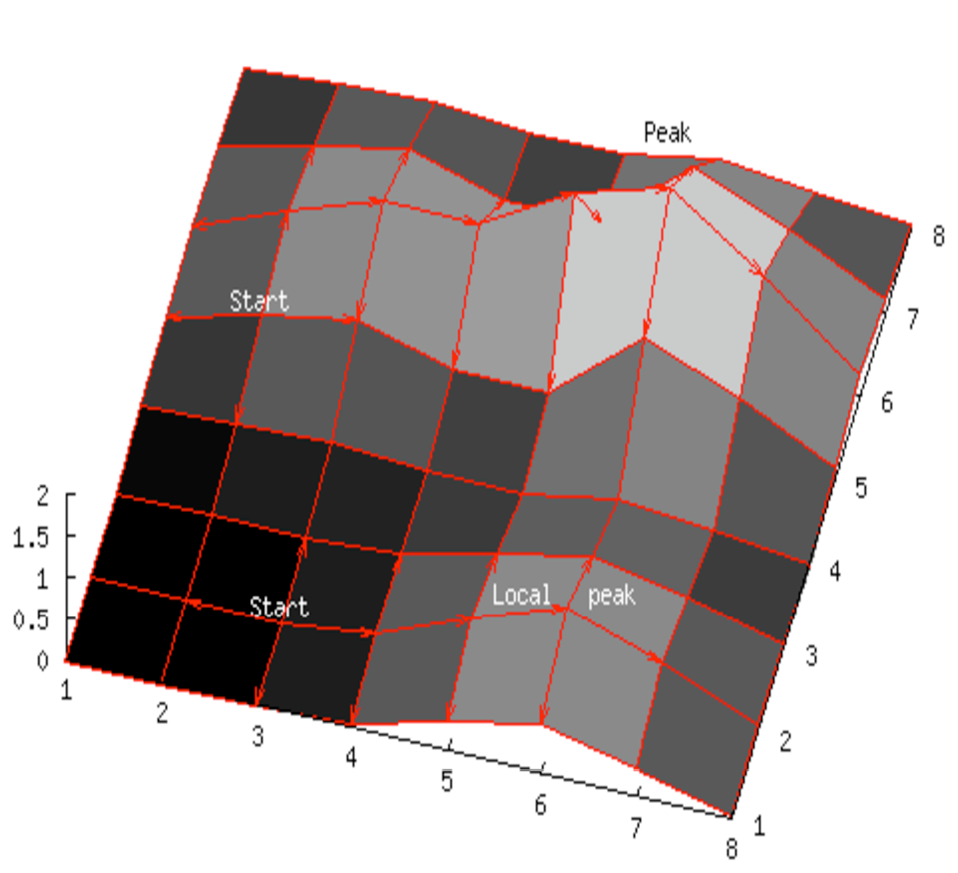
\includegraphics[width=\textwidth]{../images/hillyLandscape2}

\end{columns}

\small{}
\begin{itemize}
\item This space can be \textbf{sampled} in a Bayesian analysis with MCMC
\item The peak can be identified by a \textbf{search algorithm} in the context of maximum likelihoods
\end{itemize}

\end{frame}

